\documentclass[14pt]{extreport}
\usepackage{gost}
%\usepackage{hyperref}
%\usepackage{makecell}
\usepackage{ragged2e}

%\usepackage{graphicx}%Вставка картинок правильная
%\usepackage{float}%"Плавающие" картинки
%\usepackage{wrapfig}%Обтекание фигур (таблиц, картинок и прочего)
%\justifying

\newcolumntype{P}[1]{>{\raggedrightarraybackslash}p{#1}}
\makeatletter
\@addtoreset{figure}{part}% Reset figure numbering at every part
\makeatother
\renewcommand{\thefigure}{\arabic{figure}}% Figure number is part.figure
\renewcommand{\thetable}{\arabic{table}}

%Тут можно вставить дополнительные пакеты

\begin{document}
    \pagestyle{empty} %  выключаем нумерацию
    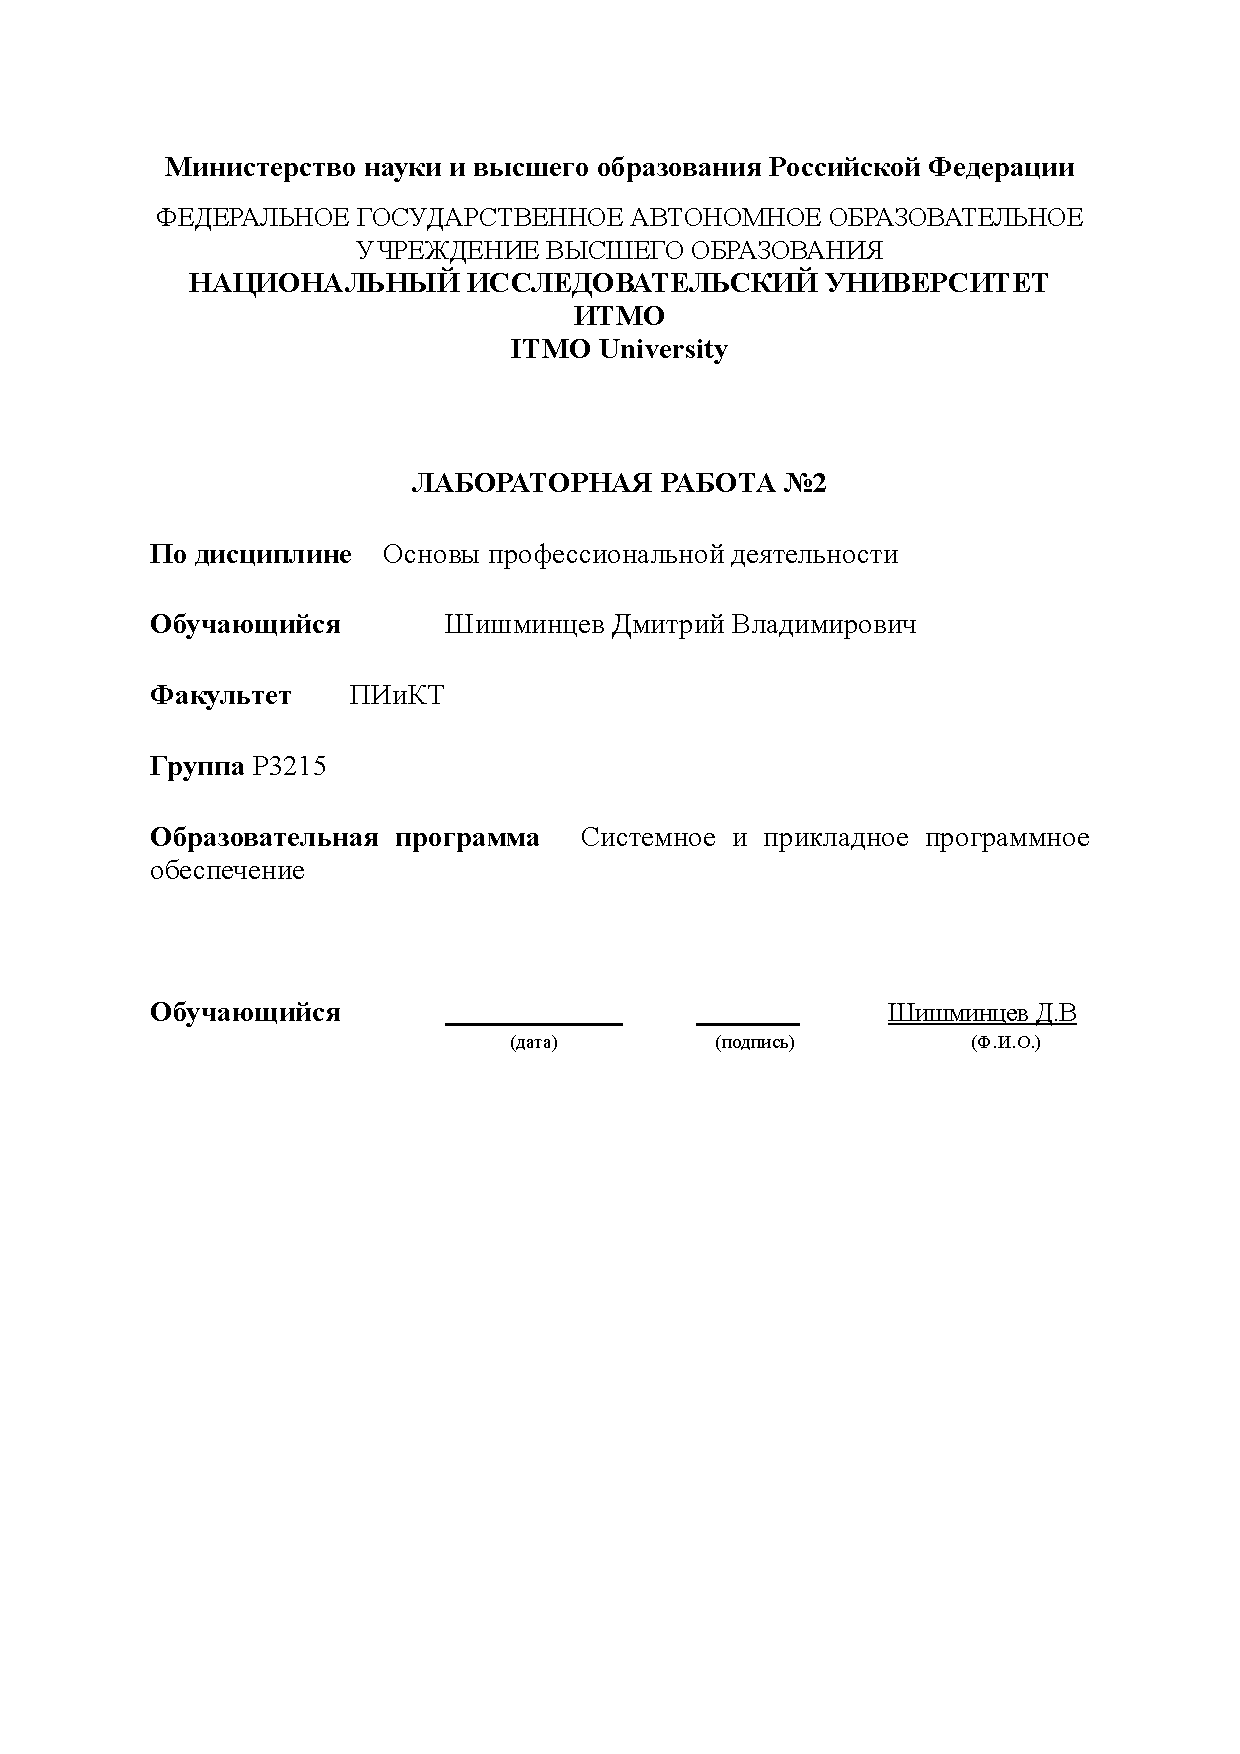
\includepdf[pages=-,pagecommand={}]{title_page.pdf}

    \pagestyle{plain} % включаем нумерацию
    \tableofcontents
    \intro Задание по базовой электронной вычислительной машине (ЭВМ) предполагает анализ программы, определение её функции, области представления и области допустимых значений исходных данных и результатов. В процессе выполнения задания требуется также провести трассировку программы и предложить вариант с уменьшенным числом команд. Этот анализ поможет понять, как программа взаимодействует с данными и как можно оптимизировать её выполнение.

    \chapter{Текст задания}


        \begin{figure}[!h]
            \centering
            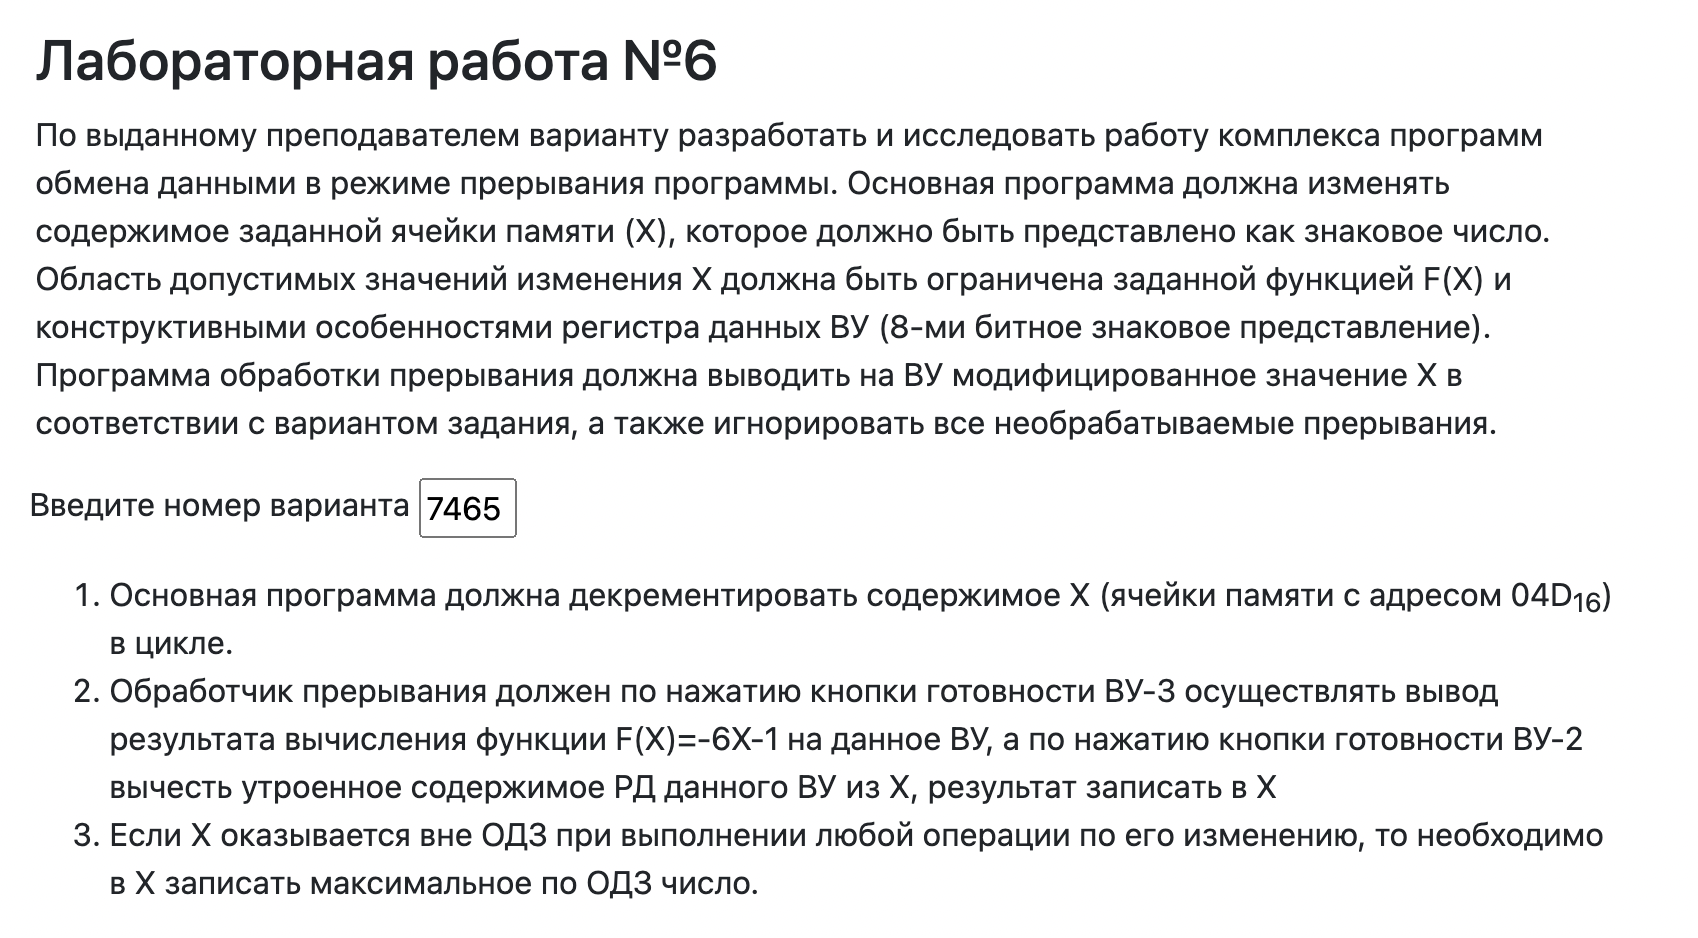
\includegraphics[width=0.8\linewidth]{task.png}
            \caption{Картинка задания}

        \end{figure}


    \chapter{Программа на языке ассемблера БЭВМ}
    \begin{verbatim}
ORG 0x0
V0: WORD $DEFAULT
    WORD 0x180
V1: WORD $DEFAULT
    WORD 0x180
V2: WORD $DEV2
    WORD 0x180
V3: WORD $DEV3
    WORD 0x180
V4: WORD $DEFAULT
    WORD 0x180
V5: WORD $DEFAULT
    WORD 0x180
V6: WORD $DEFAULT
    WORD 0x180
V7: WORD $DEFAULT
    WORD 0x180

DEFAULT: IRET

ORG 0x20
INIT:
    DI
    LD #0xA
    OUT 0x5
    LD #0xB
    OUT 0x7
    CLA
    OUT 0x1
    OUT 0x3
    OUT 0xB
    OUT 0xE
    OUT 0x12
    OUT 0x16
    OUT 0x1A
    OUT 0x1E
    EI
    JUMP MAIN

MAIN:
    LD X
    DEC
    CALL IS_IN_RANGE
    ST X
    JUMP MAIN

DEV3:
    LD X
    NEG
    ST X
    ADD X
    ADD X
    ADD X
    ADD X
    ADD X
    DEC
    OUT 6
    HLT
    IRET

IS_IN_RANGE:
    CMP MAX_RANGE
    BEQ RETURN_RANGE
    BGE RETURN_MAX
    CMP MIN_RANGE
    BGE RETURN_RANGE
    RETURN_MAX:
        LD MAX_RANGE
    RETURN_RANGE:
        RET


ORG 0x4D
X: WORD 0x15
TEMP: WORD 0x0000
MAX_RANGE: WORD 0x15
MIN_RANGE: WORD 0xFFEA

DEV2:
    IN 0x4
    SXTB
    NEG
    ST TEMP
    LD X
    ADD TEMP
    ADD TEMP
    ADD TEMP
    ST X
    HLT
    IRET
    \end{verbatim}


    \chapter{Описание программы}
    \section{Реализуемая функция}
        \textsc{ВУ-2:} $X = X - 3Y$ (y - ввод с ВУ-2) \\

        \textsc{ВУ-3:} f(x) = $-6X-1$

    \section{Область допустимых значений}
    Для переменной X: \\


        $$-21<x<21$$  \\

    \section{Расположение в памяти ЭВМ}
        0x000 - 0x00F - Векторы прерываний \\

        0x010 - Стандарт    ный обработчик прерываний \\

        0x020 - 0x02F - Инициализация векторов \\

        0x030 - 0x035 - Основная программа \\

        0x035 - 0x40 - Обработчик прерываний для ВУ-3 \\

        0x041 - 0x047 - Подпрограмма для проверки ОДЗ \\

        0x04D - Переменная Х \\

        0x04E - Временная переменная TEMP \\

        0x04F - Переменная с допустимым максимумом по ОДЗ \\

        0x050 - Переменная с допустимым минимумом по ОДЗ \\

        0x051 - 0x5A - Обработчик прерываний для ВУ-2 \\


    \chapter{Методика проверки}
        \begin{itemize}
            \item Загрузить программу в память
            \item Записать адрес старта программы в IP
            \item Запустить программу
            \item Ввести данные с помощью ВУ-2
            \item Сверить значение X
            \item Нажать на кнопку готовности ВУ-3
            \item Сверить значение
        \end{itemize}

        \bigskip
        \begin{tabular}{|c|c|c|c|}
            \hline
            ВУ & X & Ввод & Результат \\
            \hline
            ВУ-2 & 0x0001 & 0x0001 & 0xFFFE \\
            ВУ-2 & 0x0005 & 0x0003 & 0xFFFC \\
            ВУ-3 & 0x0001 && 0xFFF9 \\
            ВУ-3 & 0x0005 && 0xFFE1 \\

            \hline
        \end{tabular}

    \conclusions Исследование программы на базовой ЭВМ позволяет глубже понять её работу и оптимизировать выполнение, что важно для повышения эффективности и экономии ресурсов. Анализ функции, области представления и области допустимых значений данных, трассировка программы и оптимизация команд помогут более эффективно использовать ресурсы ЭВМ и достичь более эффективных результатов в вычислениях.

\end{document}